\addbibresource{reference.bib}

\chapter{Testování}\label{chap:test}
V této kapitol bude čtenář seznámen s metodami testování pro zajištění kvality jednotlivých softwarových komponent a s provedenými experimenty.

%********************************************************************************
% Metody testování
%********************************************************************************
\section{Metody testování}
\subsection{Jednotkové testy}
Pro části jednotlivých softwarových komponent byly použity jednotkové testy \cite{testing_evans} (tzv. \textit{Unit testy}). Jednotkové testy jsou základním typem testu, který ověřuje funkčnost samostatně testovatelných částí systému - tzv. jednotek. Výhodou těchto testů je jejich automatizovatelnost. Byl použit \textit{JUnit} framework - framework pro jednotkové testy pro platformu Java. 

\subsection{Integrační testy}
Integrační testy byly použity pro ověření správné komunikace jednotlivých komponent systému, zejména pak handlera (viz \ref{chap:handler}) a backendové aplikace mastera (viz \ref{chap:master:backend}), vyčítacího rozhraní \textit{Katherine} a komunikačního modulu apod.

V rámci těchto testů byla ověřována především správnost implementace komunikačního protokolu vyčítacího rozhraní \textit{katherine} (resp. její serverové implementace v emulátoru i implementace klienta v komunikačním modulu) a REST API handlera a mastera.

\subsection{Systémové testy}
Systémové testy se provádějí pro ověření funkčnosti systému jako celku. Tyto testy se provádějí až v pozdějších fázích vývoje a testují funkčnost systému z pohledu uživatele. Za tímto účelem bylo definováno několik testovacích scénářů (jako např. přidání detektoru do systému, přiřazení detektoru handleru, spuštění akvizice apod.), pomocí kterých byly tyto testy realizovány.

%********************************************************************************
% Experimenty
%********************************************************************************
\section{Experimenty}
Pro ověření funkčnosti a dostatečné propustnosti systému bylo provedeno několik experimentů, které budou v této podkapitole popsány. Pro tyto experimenty byla použita dvě různá prostředí:
\begin{description}
    \item[lokální] -- jeden počítač, na kterém byl spuštěn emulátor, handler a master současně. Použitý počítač má CPU 3 GHz Intel Core i7, 16 GB 1600 MHz DDR3 RAM a SSD disk o kapacitě \unit{500}{GB} (MacBook Pro).
    \item[CERN openstack] -- cloudová infrastruktura v CERN, kterou CERN poskytuje partnerským univerzitám a dalším institucím. Tato infrastruktura je založená na \textit{OpenStack} \textit{IaaS}\footnote{Z angl. \textit{Infrastructure as a Service}.} platformě, která umožňuje řízení výpočetního výkonu, úložiště a síťových prostředcích v datacentrech skrze webovou aplikaci nebo \textit{OpenStack API}.

    Byl vytvořen cluster s těmito virtuálními počítači:
    \begin{itemize}
        \item \texttt{pixnet-master.cern.ch} -- na tomto uzlu byla nasazena backendová aplikace mastera společně s webovým serverem, poskytujícím webový frontend mastera. Instance má 2~VCPU, \unit{4}{GB}~RAM a \unit{20}{GB} diskové kapacity.
        \item \texttt{pixnet-handler-1.cern.ch} -- uzel pro nasazení backendové aplikace handlera. Instance má 4~VCPU, \unit{8}{GB}~RAM a \unit{40}{GB} diskové kapacity.
        \item \texttt{pixnet-emulator-katherine1.cern.ch} -- uzel pro nasazení emulátoru vyčítacího rozhraní \textit{Katherine}. Instance má 1~VCPU, \unit{2}{GB}~RAM a \unit{10}{GB} diskové kapacity.
        \item \texttt{pixnet-emulator-katherine2.cern.ch} -- uzel pro nasazení emulátoru vyčítacího rozhraní \textit{Katherine}. Instance má 1~VCPU, \unit{2}{GB}~RAM a \unit{10}{GB} diskové kapacity.
    \end{itemize}

\end{description}

%********************************************************************************
% Experimenty - Experiment první
%********************************************************************************
\subsection{Experiment první: zpracovávání fronty naměřených dat}
Kritickou částí každého datového akvizičního systému je proces zpracování dat, od přijetí až po jejich uložení. Jelikož v rámci systému Pixnet data procházejí pouze přes handler (resp. od komunikačního do datového modulu daného detektoru, zavedených v handleru) do datovým modulem definovaného úložiště, budou v rámci tohoto experimentu zkoumány jen metadata jednotlivých událostí (od jejich vzniku až po uložení).

Experiment byl proveden v obou prostředích, v každém s jedním emulátorem vyčítacího rozhraní \textit{Katherine}, jedním handlerem a masterem. Byly sledovány dva parametry - čas zpracování události (tj. doba od jeho přijetí komunikačním modulem až po jeho uložení datovým modulem) a aktuální počet událostí ve frontě. Pro všechna měření byl emulátor nastaven tak, aby generoval fixní počet událostí za sekundu. Jako vyčítací mód emulátoru byl použit \textit{Data-Driven} (viz \ref{chap:detectors:readout}), akviziční mód byl \textit{ToA \& TOT} a délka akvizice byla vždy \unit{60}{s}. Na obr. \ref{fig:test:exp1:jedna_akvizice_50k_udalosti} je znázorněn průběh jednoho měření, při kterém emulátor generoval 50000 událostí za vteřinu, který zaznamenává vývoj doby zpracovávání událostí a velikosti fronty v čase.

\begin{figure}[h]
    \centering
    \begin{tikzpicture}
        \begin{axis}[
          xmin = 0, xmax = 62000,
          ymin = 0,
          axis y line*=left,
          xlabel={Čas [ms]},
          xlabel near ticks,
          ylabel={Doba zpracování událostí [ns]},
          ylabel near ticks,
          width=0.90\textwidth,
          height=0.89\textwidth,
        ]
          \addplot[color=orange] table {figures/data/test_queue_waiting.dat};
          \label{plot_1_y1}
        \end{axis}
        \begin{axis}[
          xmin = 0, xmax = 62000,
          ymin = 0,% ymax = 11000,
          hide x axis,
          axis y line*=right,
          ylabel={Počet událostí ve frontě},
          ylabel near ticks,
          width=0.90\textwidth,
          height=0.89\textwidth,
        ]
        \addplot[color=gray] table {figures/data/test_queue_size.dat};
        \label{plot_1_y2}
        \addlegendimage{/pgfplots/refstyle=plot_1_y1}\addlegendentry{Doba zpracování událostí}
        \addlegendimage{/pgfplots/refstyle=plot_1_y2}\addlegendentry{Počet událostí ve frontě}
        \end{axis}
      \end{tikzpicture}

    \caption{Vývoj doby zpracovávání událostí a počtu událostí ve frontě v rámci \unit{60}{s} dlouhé akvizice, při konstantním generovaném množství událostí ($50000~s^{-1}$).}
    \label{fig:test:exp1:jedna_akvizice_50k_udalosti}
\end{figure}

Měření byla provedena pro různé počty generovaných událostí za vteřinu (1, 10, 100, 1000, 10000, 25000, 50000, 75000 a 100000), ze kterých byla stanovena průměrná doba zpracovávání události v závislosti na počtu příchozích dat (viz obr. \ref{fig:test:exp1:zavyslost_na_poctu_udalosti:doba_zpracovani}) a průměrná velikost fronty v závislosti na počtu příchozích dat (viz obr. \ref{fig:test:exp1:zavyslost_na_poctu_udalosti:velikost_fronty}). Jednotlivá měření byla vícekrát zopakována a jejich dílčí hodnoty byly zprůměrovány. Maximální testovaný počet generovaných událostí za vteřinu byl 100000, kvůli omezení emulátoru.

\begin{figure}[h]
    \centering
    \begin{subfigure}[t!]{0.47\textwidth}
        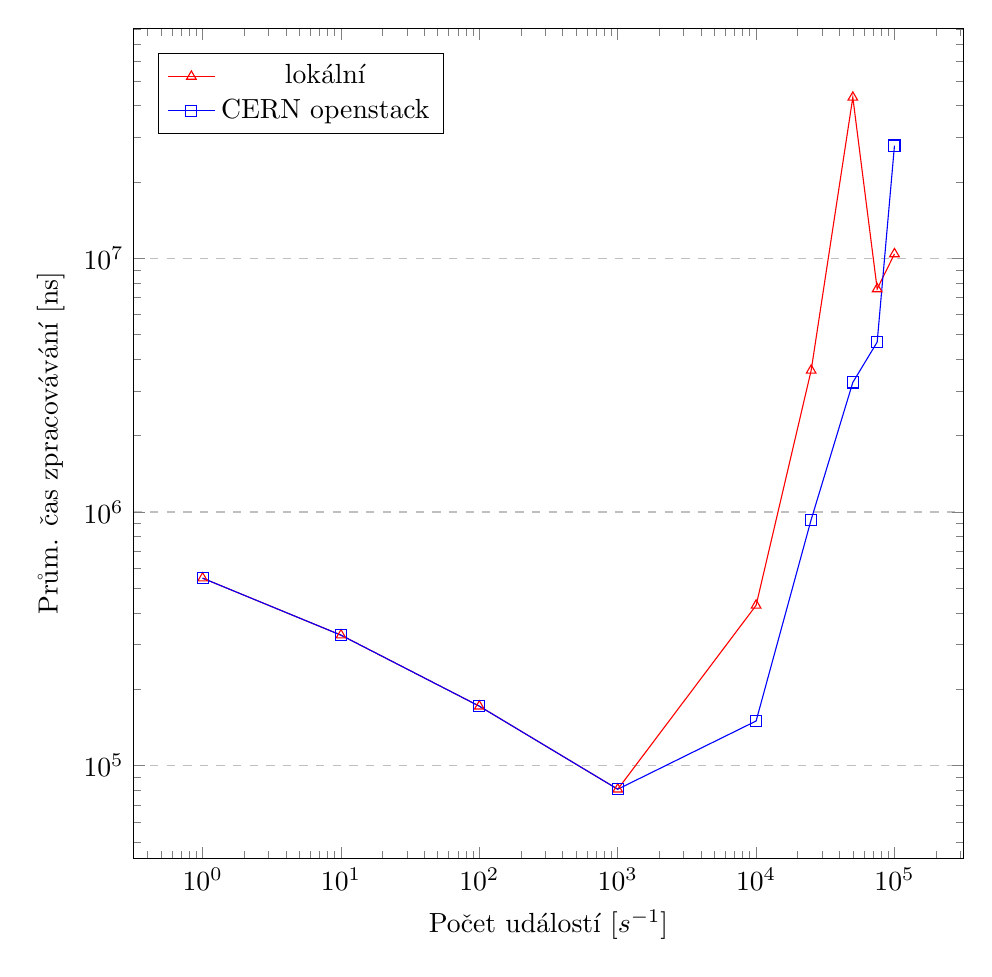
\begin{tikzpicture}
            \begin{loglogaxis}[
                xlabel={Počet událostí [$s^{-1}$]},
                ylabel={Prům. čas zpracovávání [ns]},
                legend pos=north west,
                ymajorgrids=true,
                grid style=dashed,
                width=\textwidth,
                height=\textwidth,
            ]
            \addplot[
                color=red,
                mark=triangle,
                ]
                coordinates {
                    (1,548539.5)
                    (10,327037.6097)
                    (100,171609.3892)
                    (1000,80747.81636)
                    (10000,428631.4967)
                    (25000,3616756.103)
                    (50000,43089381.58)
                    (75000,7572697.545)
                    (100000,10406080.54)
                };
            \addplot[
                color=blue,
                mark=square,
                ]
                coordinates {
                    (1,548539.5)
                    (10,327037.6097)
                    (100,171609.3892)
                    (1000,80747.81636)
                    (10000,150000.808)
                    (25000,933122.5602)
                    (50000,3242140.3333)
                    (75000,4674643.645)
                    (100000,27828674.3)
                };
            \legend{lokální,CERN openstack} 
            \end{loglogaxis}
        \end{tikzpicture}
        \caption{Závislost průměrné doby zpracování události na počtu událostí za sekundu.}
        \label{fig:test:exp1:zavyslost_na_poctu_udalosti:doba_zpracovani}
    \end{subfigure}
    \hspace{0.2cm}
    \begin{subfigure}[t!]{0.47\textwidth}
    
        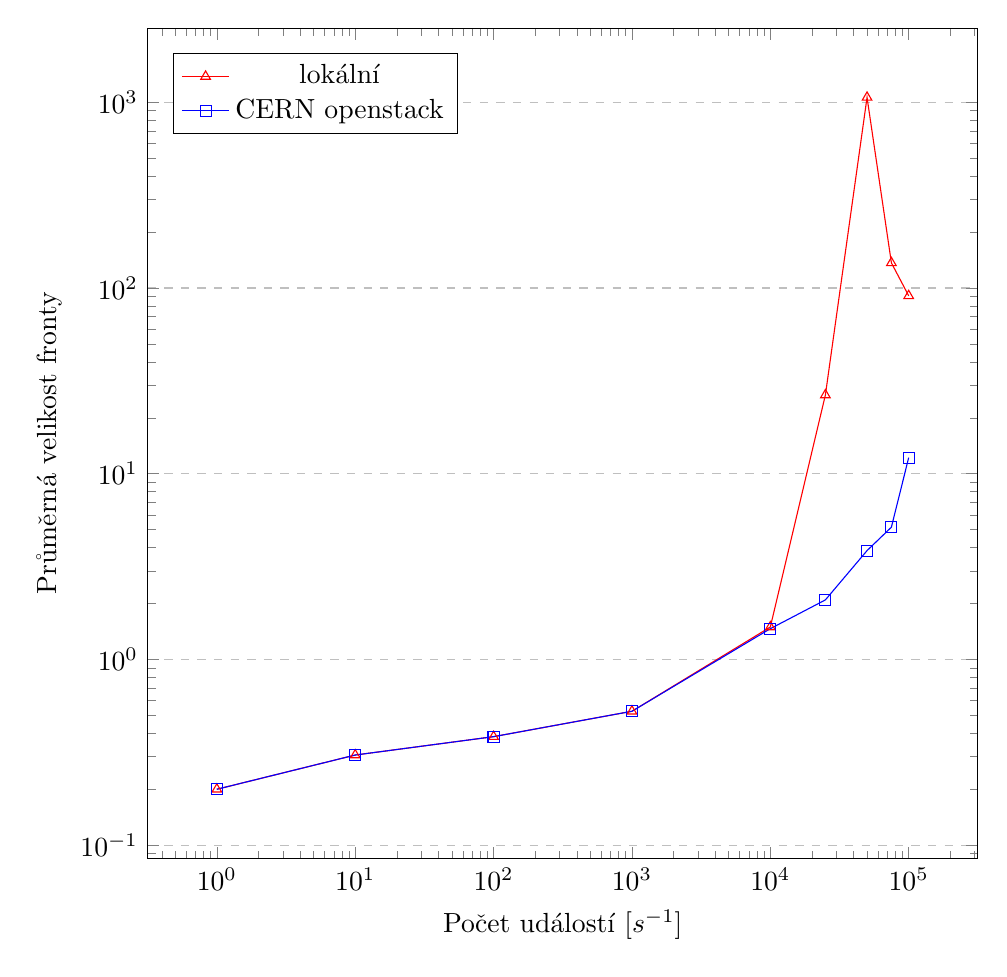
\begin{tikzpicture}
            \begin{loglogaxis}[
                xlabel={Počet událostí [$s^{-1}$]},
                ylabel={Průměrná velikost fronty},
                legend pos=north west,
                ymajorgrids=true,
                grid style=dashed,
                width=\textwidth,
                height=\textwidth,
            ]
            \addplot[
                color=red,
                mark=triangle,
                ]
                coordinates {
                    (1,0.2)
                    (10,0.305699482)
                    (100,0.383944154)
                    (1000,0.525876461)
                    (10000,1.495)
                    (25000,26.53898305)
                    (50000,1061.88027)
                    (75000,136.5602007)
                    (100000,90.73529412)
                };
            \addplot[
                color=blue,
                mark=square,
                ]
                coordinates {
                    (1,0.2)
                    (10,0.305699482)
                    (100,0.383944154)
                    (1000,0.525876461)
                    (10000,1.464106845)
                    (25000,2.091973244)
                    (50000,3.854271357)
                    (75000,5.154103853)
                    (100000,12.20805369)
                };
            \legend{lokální,CERN openstack}
            \end{loglogaxis}
        \end{tikzpicture}
        \caption{Závislost průměrné velikosti fronty s událostmi na počtu událostí za sekundu.}
        \label{fig:test:exp1:zavyslost_na_poctu_udalosti:velikost_fronty}
        
    \end{subfigure}
        
    \caption{Závislost průměrné doby zpracování událostí a jejich průměrného počtu ve frontě na počtu událostí za sekundu.}
    \label{fig:test:exp1:zavyslost_na_poctu_udalosti}
\end{figure}

Z výsledku experimentu je patrné, že obě sledované hodnoty rostou s počtem událostí. Oproti očekávaným hodnotám (resp. očekávané rostoucí závislosti) lze z obr. \ref{fig:test:exp1:zavyslost_na_poctu_udalosti} pozorovat dva rozdíly. 

Tím prvním je vývoj průměrné doby zpracování události od jedné do 1000 událostí za sekundu. Tento efekt je pravděpodobně způsoben nastavenou velikostí \textit{bufferu} a režie přenosu dat.

Druhým rozdílem je různý trend hodnot pro \textit{CERN openstack} a \textit{lokání} prostředí od 50000 událostí za vteřinu. Nejvíce pravděpodobnou příčinou tohoto jevu je rozdílná konfigurace obou prostředí. Zatímco v rámci \textit{CERN openstack} každá komponenta systémů je spuštěna na jiném počítači, v \textit{lokální} prostředí všechny komponenty sdílí stejný počítač a vzájemně se ovlivňují.

%********************************************************************************
% Experimenty - Experiment druhý
%********************************************************************************
\subsection{Experiment druhý: zátěžový test API mastera}
V rámci tohoto experimentu byl proveden zátěžový test API mastera. Pomocí software \textit{Apache JMeter} bylo provedeno několik měření, ve kterých byl sledován průměrný čas zpracovávání requestu (resp. jeho průměr, medián a směrodatná odchylka) a průměrný počet zpracovaných událostí za minutu v závislosti na počtu simultánně přistupujících uživatelů. Experiment byl proveden pro 1, 10, 100, 500, 1000, 2000, 3000, 4000, 5000, 6000, 7000, 8000, 9000 a 10000 uživatelů, resp. použitých vláken. Každý experiment byl několikrát zopakován a výsledky byly zprůměrovány. 

Výsledek experimentu je zobrazen v obrázku \ref{fig:test:exp2}. Z grafu je patrné, že do zhruba 3000 simultánně přistupujících uživatelů počet zpracovaných uživatelů za minutu stoupá

\begin{figure}[h]
    \centering
    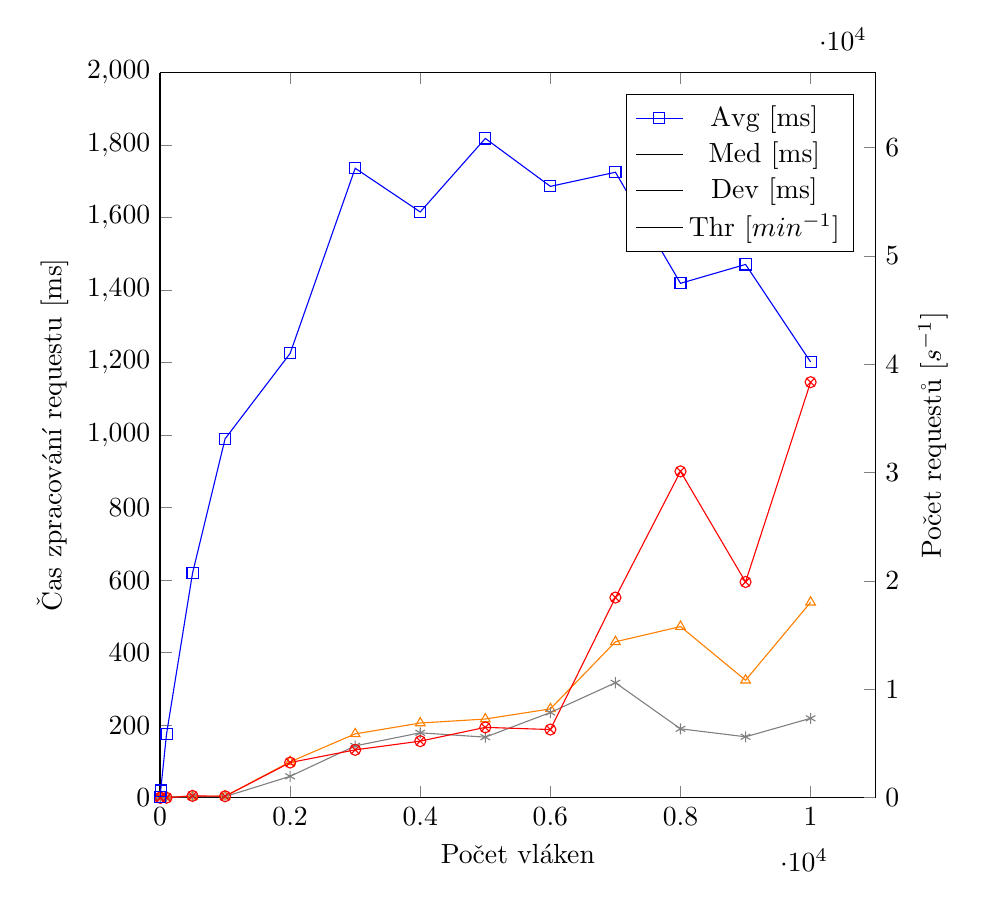
\begin{tikzpicture}
        \begin{axis}[
          xmin = 0,% xmax = 62000,
          ymin = 0, ymax = 2000,
          axis y line*=left,
          xlabel={Počet vláken},
          xlabel near ticks,
          ylabel={Čas zpracování requestu [ms]},
          ylabel near ticks,
          width=0.88\textwidth,
          height=0.89\textwidth,
        ]
            \addplot[color=orange,mark=triangle]
                coordinates {
                    (1,3)
                    (10,2)
                    (100,2)
                    (500,4)
                    (1000,4)
                    (2000,99)
                    (3000,176)
                    (4000,206)
                    (5000,217)
                    (6000,245)
                    (7000,430)
                    (8000,472)
                    (9000,324)
                    (10000,539)
                };
            \label{plot_2_y1}
            \addplot[color=gray,mark=asterisk]
                coordinates {
                    (1,3)
                    (10,2)
                    (100,2)
                    (500,3)
                    (1000,3)
                    (2000,59)
                    (3000,143)
                    (4000,179)
                    (5000,167)
                    (6000,235)
                    (7000,317)
                    (8000,190)
                    (9000,168)
                    (10000,219)
                };
            \label{plot_2_y2}
            \addplot[color=red,mark=otimes]
                coordinates {
                    (1,0)
                    (10,0)
                    (100,0)
                    (500,5)
                    (1000,4)
                    (2000,97)
                    (3000,132)
                    (4000,156)
                    (5000,194)
                    (6000,188)
                    (7000,552)
                    (8000,900)
                    (9000,595)
                    (10000,1146)
                };
            \label{plot_2_y3}
        \end{axis}
        \begin{axis}[
          xmin = 0,% xmax = 62000,
          ymin = 0,% ymax = 11000,
          hide x axis,
          axis y line*=right,
          ylabel={Počet requestů [$s^{-1}$]},
          ylabel near ticks,
          width=0.88\textwidth,
          height=0.89\textwidth,
          legend pos=north east,
        ]
        \addplot[color=blue,mark=square]
                coordinates {
                    (1,53)
                    (10,662)
                    (100,5870)
                    (500,20732)
                    (1000,33127)
                    (2000,41011)
                    (3000,58100)
                    (4000,54066)
                    (5000,60851)
                    (6000,56426)
                    (7000,57731)
                    (8000,47477)
                    (9000,49222)
                    (10000,40222)
                };
            \label{plot_2_y4}

        %\label{plot_2_y2}
        \addlegendimage{/pgfplots/refstyle=plot_2_y1}\addlegendentry{Avg [ms]}
        \addlegendimage{/pgfplots/refstyle=plot_2_y2}\addlegendentry{Med [ms]}
        \addlegendimage{/pgfplots/refstyle=plot_2_y3}\addlegendentry{Dev [ms]}
        \addlegendimage{/pgfplots/refstyle=plot_2_y4}\addlegendentry{Thr [$min^{-1}$]}
        \end{axis}
      \end{tikzpicture}

    \caption{Závislost počtu zpracovávaných requestů za minutu (v legendě jako \textit{Thr}, pravá osa) na počtu vláken a závislost času zpracovávání requestu (znázorněno jako \textit{Avg} (průměr), \textit{Med} (medián) a \textit{Dev} (směrodatná odchylka), levá osa) na počtu vláken.}
    \label{fig:test:exp2}
\end{figure}